%%%%%%%% ICML 2026 EXAMPLE LATEX SUBMISSION FILE %%%%%%%%%%%%%%%%%

\documentclass{article}

% Recommended, but optional, packages for figures and better typesetting:
\usepackage{microtype}
\usepackage{graphicx}
\usepackage{subcaption}
\usepackage{booktabs} % for professional tables

\usepackage{float}  % 必须加载，[H]参数依赖此宏包

\usepackage{amsmath}
\usepackage{amssymb}
\usepackage{mathtools}
\usepackage{amsthm}
\usepackage{algorithm}
\usepackage{algorithmic}
\usepackage{xcolor} % 用于颜色注释

\usepackage{booktabs}
\usepackage{multirow}
\usepackage[table]{xcolor} % 必须加上 [table] 选项
\usepackage{amsmath}       % 用于下箭头符号
\usepackage{pifont}
\usepackage{enumitem} 
% 定义图片中的近似颜色
\definecolor{tspgreen}{RGB}{226, 240, 217} % TSP部分的浅绿色
\definecolor{cvrpblue}{RGB}{221, 243, 250} % CVRP部分的浅蓝色


% hyperref makes hyperlinks in the resulting PDF.
% If your build breaks (sometimes temporarily if a hyperlink spans a page)
% please comment out the following usepackage line and replace
% \usepackage{icml2026} with \usepackage[nohyperref]{icml2026} above.
\usepackage{hyperref}


% Attempt to make hyperref and algorithmic work together better:


% Use the following line for the initial blind version submitted for review:
%\usepackage{icml2026}

% For preprint, use
\usepackage{icml2026}

% If accepted, instead use the following line for the camera-ready submission:
% \usepackage{icml2026}



 

% if you use cleveref..
\usepackage[capitalize,noabbrev]{cleveref}

%%%%%%%%%%%%%%%%%%%%%%%%%%%%%%%%
% THEOREMS
%%%%%%%%%%%%%%%%%%%%%%%%%%%%%%%%
\theoremstyle{plain}
\newtheorem{theorem}{Theorem}[section]
\newtheorem{proposition}[theorem]{Proposition}
\newtheorem{lemma}[theorem]{Lemma}
\newtheorem{corollary}[theorem]{Corollary}
\theoremstyle{definition}
\newtheorem{definition}[theorem]{Definition}
\newtheorem{assumption}[theorem]{Assumption}
\theoremstyle{remark}
\newtheorem{remark}[theorem]{Remark}

% Todonotes is useful during development; simply uncomment the next line
%    and comment out the line below the next line to turn off comments
%\usepackage[disable,textsize=tiny]{todonotes}
\usepackage[textsize=tiny]{todonotes}

% The \icmltitle you define below is probably too long as a header.
% Therefore, a short form for the running title is supplied here:
\icmltitlerunning{Submission and Formatting Instructions for ICML 2026}

\begin{document}

\twocolumn[
  \icmltitle{Rethink Efficiency Side of Neural Combinatorial Solver: \\ An Offline and Self-Play Paradigm}

  % It is OKAY to include author information, even for blind submissions: the
  % style file will automatically remove it for you unless you've provided
  % the [accepted] option to the icml2026 package.

  % List of affiliations: The first argument should be a (short) identifier you
  % will use later to specify author affiliations Academic affiliations
  % should list Department, University, City, Region, Country Industry
  % affiliations should list Company, City, Region, Country

  % You can specify symbols, otherwise they are numbered in order. Ideally, you
  % should not use this facility. Affiliations will be numbered in order of
  % appearance and this is the preferred way.
  \icmlsetsymbol{equal}{*}

  \begin{icmlauthorlist}\icmlauthor{Anonymous}{anon}\end{icmlauthorlist}

  \icmlaffiliation{anon}{Anonymous Institution}
  
  % 
  

  \icmlcorrespondingauthor{Anonymous}{anonymous@anonymous.invalid}


  % You may provide any keywords that you find helpful for describing your
  % paper; these are used to populate the "keywords" metadata in the PDF but
  % will not be shown in the document
  \icmlkeywords{Machine Learning, ICML}

  \vskip 0.3in
]

% this must go after the closing bracket ] following \twocolumn[ ...

% This command actually creates the footnote in the first column listing the
% affiliations and the copyright notice. The command takes one argument, which
% is text to display at the start of the footnote. The \icmlEqualContribution
% command is standard text for equal contribution. Remove it (just {}) if you
% do not need this facility.

% Use ONE of the following lines. DO NOT remove the command.
% If you have no special notice, KEEP empty braces:
\printAffiliationsAndNotice{}  % no special notice (required even if empty)
% Or, if applicable, use the standard equal contribution text:
% \printAffiliationsAndNotice{\icmlEqualContribution}

\begin{abstract}
We propose ECO, a versatile learning paradigm that enables efficient offline self-play for Neural Combinatorial Optimization (NCO). ECO addresses key limitations in the field through: 1) \emph{Paradigm Shift}: Moving beyond inefficient online paradigms, we introduce a two-phase offline paradigm consisting of supervised warm-up and iterative Direct Preference Optimization (DPO); 2) \emph{Architecture Shift}: We deliberately design a Mamba-based architecture to further enhance the efficiency in the offline paradigm; and 3) \emph{Progressive Bootstrapping}: To stabilize training, we employ a heuristic-based bootstrapping mechanism that ensures continuous policy improvement during training. Comparison results on TSP and CVRP highlight that ECO performs competitively with up-to-date baselines, with significant advantage on the efficiency side in terms of memory utilization and training throughput.  We provide further in-depth analysis on the efficiency, throughput and memory usage of ECO. Ablation studies show rationale behind our designs. 

%Our code is available at \href{https://anonymous.4open.science/r/ECO-F7BD/}{https://anonymous.4open.science/r/ECO-F7BD/}.
\end{abstract}
\vspace{-20pt}
\section{Introduction}
Combinatorial Optimization (CO) is essential for domains such as chip design~\cite{chip-design}, routing~\cite{routing}, supply chain~\cite{supply-chain}, logistics~\cite{logistic} and scheduling~\cite{scheduling}. Over the past decades, how to solve CO has been discussed and explored extensively, and representative legacy such as Concorde~\cite{concorde2006}, Lin-Kernighan-Helsgaun algorithm~\cite{lkh}, ant system~\cite{ant}, genetic algorithm~\cite{ga} more or less address CO's complexity. However, these meta-heuristics closely depend on expert-level knowledge to be crafted or even customized per case. As foretold by \emph{no-free-lunch} theorem~\cite{no-free-lunch}, such dependency may result in limited adaptability and scalability across diverse CO problems.


Learning-based approaches are continuously getting popular more recently for dealing with complex CO problems~\cite{nco-2016-start}, which are commonly termed as Neural Combinatorial Optimization (NCO). Along NCO's development, a crystal clear evolution path on the performance side could be observed from recent advances in this field:  from pointer network~\cite{1} to Transformer architecture~\cite{transformer} and Generative Flow Network~\cite{flow-network}, from normal scale case~\cite{3} to massive scale generalization~\cite{boosting} and from simple reinforcement learning~\cite{4} to enhanced hybrid training~\cite{GFlowNet}. In contrast, to the best of our knowledge, limited attention is paid to the efficiency side~\cite{efficient-nco-1,efficient-nco-2}. This induces the core motivation of this paper: what should be done to achieve efficient NCO learning? This is a quite important question since efficiency impacts multi-dimensional aspects in NCO, such as learning effectiveness, scalability and practical application value.

% Neural Combinatorial Optimization (NCO) offers a data-driven alternative, evolving from pointer network~\cite{} to Transformer architecture~\cite{}. However, current NCO methods struggle with scalability despite their effectiveness on small instances.

Following the first principle, the efficiency bottleneck of existing NCO works predominantly roots from two aspects: 1) \textbf{Learning Paradigm}: The rollout and training in existing works compose an online paradigm. Such sampling-then-training mode hardly benefits from parallelization and holistic GPU utilization; 2) \textbf{Neural Network Architecture}: State-of-the-art NCO models predominantly rely on the Transformer architecture~\cite{transformer}, the core self-attention mechanism incurs quadratic computational and memory costs. Clearly, this field anticipates an effective framework to address these efficiency issues.


To address this, we propose an efficient NCO framework pertinently, termed as \textbf{ECO}, to enable cost-effective training of neural solvers through shifts of both the learning paradigm and the neural network architecture. Specifically, we first turn the learning paradigm from existing online fashion toward offline learning paradigm~\cite{offline-1,offline-2}. A two-phase training workflow is carefully established, where the first phase utilizes high quality offline trajectories and supervised training to assure quick warm-up, and the second phase adopts Direct Preference Optimization~(DPO)~\cite{10} to further refine the model with self-play and contrastive update. To further benefit from such offline paradigm, we propose a tailored network architecture based on Mamba~\cite{mamba}, a selective state space model. Without changing the autoregressive sampling paradigm, the proposed architecture improve the overall throughput and scalability via hardware-aware parallel scanning and efficient recurrent kernels. As illustrated in Figure \ref{fig:intro}, by combining the high-throughput Mamba architecture with a stable offline DPO training scheme, ECO achieves superior convergence speed and stability, reaching high-quality solutions significantly faster than varying baselines under the same hardware constraints. Our contributions are in three-folds:

\begin{figure}[t]  % 核心修改：[!ht]替代[H]
\centering
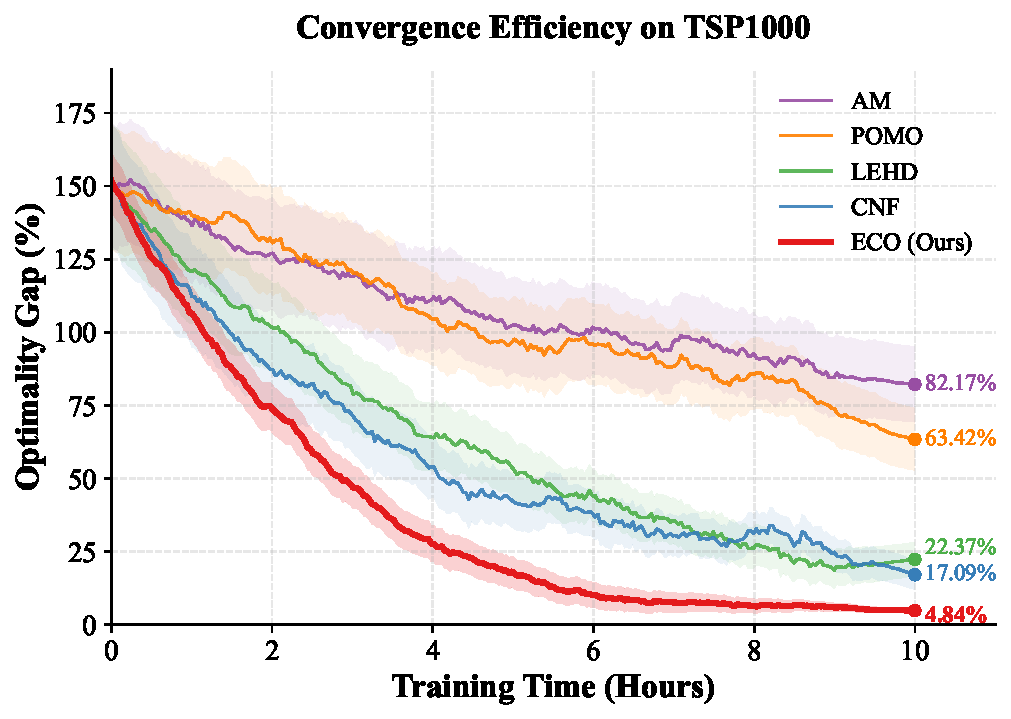
\includegraphics[width=0.85\linewidth]{figure/convergence.pdf}
\vspace{-5pt}
\caption{Convergence efficiency on TSP1000. The curves display the average optimality gap over 20 independent runs, with shaded regions indicating the standard deviation. All methods were trained on a single NVIDIA A800 GPU, with batch sizes tuned to maximize hardware utilization for each respective model.}
\label{fig:intro}
\vspace{-5pt}
\end{figure}

% State-of-the-art NCO models predominantly rely on the Transformer architecture and On-Policy Reinforcement Learning (RL), creating a dual barrier to advancement:

% \textbf{Architectural Bottleneck ($O(N^2)$ Complexity):} The core self-attention mechanism incurs quadratic computational and memory costs. As problem size $N$ scales to thousands, GPU memory limitations and inference latency become prohibitive. Furthermore, positional embeddings in Transformers often struggle with Out-of-Distribution (OOD) generalization, leading to performance degradation on instances larger than those seen during training.

% \textbf{Training Bottleneck (Sample Inefficiency):} Standard training paradigms, such as REINFORCE with greedy rollouts, are inherently on-policy. They necessitate expensive autoregressive sampling within the training loop, preventing parallelization and leading to low GPU utilization. Moreover, the sparse and delayed rewards in CO induce high variance in gradient estimation, destabilizing convergence—particularly for large-scale graphs.

% To dismantle these barriers, we propose a cohesive framework that synergizes the linear complexity of Mamba with the stability of Iterative Direct Preference Optimization (DPO).

% First, we address the architectural constraint by adapting Mamba, a Selective State Space Model (SSM), for NCO. Unlike Transformers, Mamba leverages a hardware-aware Parallel Scan algorithm to achieve linear time complexity $O(N)$ while maintaining global receptive fields. This shift allows us to process instances an order of magnitude larger than previous baselines under identical resource constraints. Crucially, Mamba’s recurrent inductive bias inherently facilitates superior length extrapolation.

% Second, we transition from on-policy RL to an offline preference-based framework. We adapt Direct Preference Optimization, originally designed for LLM alignment, to the structured domain of combinatorial problems. Instead of maximizing scalar rewards via unstable policy gradients, we construct preference pairs contrasting superior solutions $y_w$ with inferior ones $y_l$. The policy is then optimized to distinguish between these pairs. To mitigate distribution shift, we introduce Iterative DPO. This closed-loop process of self-sampling, preference construction, and offline updates enables continuous improvement via self-play without expert supervision.

% Our contributions are summarized as follows:
\begin{itemize}[leftmargin=*]
\vspace{-10pt}
    \item[\ding{182}]  We claim our ECO as a very first exploration on introducing high throughput architecture~(Mamba) and offline learning paradigm~(DPO) to NCO.
    \vspace{-7pt}
    % \textbf{Linear-Complexity Architecture:} We introduce the first Mamba-based NCO solver that breaks the quadratic complexity barrier, enabling efficient training and inference on large-scale TSP instances.
    \item[\ding{183}]  We introduce several novel designs to achieve effective and efficient offline NCO learning, which includes a tailored Mamba architecture compatible with NCO setting, and a two-phase offline training paradigm with a heuristic-based bootstrapping to ensure quick warm-up and smooth policy improvement.
    \vspace{-7pt}
    % \textbf{Stable Offline Training:} We propose Iterative DPO for NCO, eliminating the computational overhead of on-policy rollouts and mitigating the gradient variance issues inherent in traditional RL.
    \item[\ding{184}]  We conduct case study on TSP and CVRP, where rigorous benchmarking results demonstrate ECO's competitive performance and significant efficiency advantage against online NCO baselines. Ablation studies underscore the efficacy of our proposed designs.
    \vspace{-7pt}
    % \textbf{Superior Scalability and Performance:} Our framework achieves SOTA results. Extensive experiments demonstrate that our method not only converges significantly faster than Transformer-based baselines but also exhibits robust generalization capabilities on unseen problem sizes.
\end{itemize}

\section{Related Works}
\vspace{-5pt}
\subsection{Neural Combinatorial Optimization and Scalability Bottlenecks}
\vspace{-5pt}
NCO has emerged as a prominent paradigm for solving NP-hard problems such as the TSP. Early approaches, such as Pointer Networks \cite{1}, utilized RNNs to manage variable output dictionaries, while Bello et al. \cite{2} subsequently introduced reinforcement learning (RL) to enable unsupervised training. The Attention Model (AM) by Kool et al. \cite{3} established the dominance of Transformers in NCO, a framework later stabilized by POMO \cite{4} through the exploitation of solution symmetries for robust RL training. Although recent works like LEHD \cite{5} attempt to alleviate computational loads via encoder-decoder decomposition, attention-based methods remain constrained by $O(N^2)$ quadratic complexity. This creates a dual challenge of memory explosion and excessive inference latency when generalizing to large-scale instances (where $N \ge 10,00$). Consequently, developing global modeling architectures with linear complexity is a critical imperative for advancing the field of NCO.
\vspace{-10pt}
\subsection{Sequence Modeling via Mamba}\label{sec:2.2}
Recently, structured state-space~(SSM) models has been recognized as an effective alternative sequence models~\cite{6,ssm-gu,h3,linear-attn,retnet}. For an input sequence $x \in \mathbb{R}^{L \times D}$ with time horizon $L$ and $D$-dimensional signal channels at each time step, SSM processes it by the following first-order dynamic equation, which maps the input signal $x(t) \in \mathbb{R}^D$ to the time-dependent output $y(t) \in \mathbb{R}^D$ through hidden state $h(t)$ as follows:
\begin{equation}\label{eq:s4}
    h(t) = \overline{A} h(t-1) + \overline{B} x(t),\quad y(t) = C h(t).
\end{equation}
Here, $A$, $B$ and $C$ are learnable parameters, $\overline{A}$ and $\overline{B}$ are obtained by applying zero-order hold~(ZOH) discretization rule to the continuous parameters $A$ and $B$ to embrace the discrete nature in sequence-to-sequence tasks. The SSM models that fall into this paradigm is normally named as structured state-space sequence~(S4) models. We note that S4 paradigm shows beautiful properties in both the training efficiency and inference efficiency sides. For training, suppose we have an input sequence $X = [x(1),x(2),...,x(T)]$, S4 model supports ``global convolution'', which pre-computes all intermediate parameters and processes $X$ as:
\begin{equation}\label{eq:s4-kernal}
    \overline{K} = (C\overline{B},C\overline{AB},C\overline{A}^2\overline{B},...),\quad Y = X\cdot \overline{K}.
\end{equation}
This parallel training mode makes S4 models particularly advantageous in offline training settings where all data is accessible. For inference side, S4 models follows ``linear recurrence'' model in Eq.~\ref{eq:s4}, which is also economic since only constant level cache is required.

Despite its high-efficiency computation, S4 models fall shorts in time-dependent sequence modeling since the parameters are invariant for all time steps. More recently, Mamba~\cite{mamba,mamba2} is proposed as a novel SSM models, which address this issue by selective mechanism~(hence, it is also termed as S6 model), making learnable parameters time-dependent. Specifically, Mamba lets the parameters $\overline{A}$, $\overline{B}$ and $C$ be functions of the input $x(t)$. Therefore, the system now supports time-varying sequence modeling. However, such novelty sacrifices the efficient computation in S4's training since the time-dependent parameters cannot be pre-computed using the convolution mode. To mitigate this issue, Mamba borrows ideas from the prefix-sum scan algorithm to relieve complexity in recurrent mode and popular GPU memory optimization techniques. In the rest of this paper, we use S4 to denote time-invariance SSMs and use S6 to denote Mamba. 

\begin{figure*}[!ht]  % 核心修改：[!ht]替代[H]
\centering
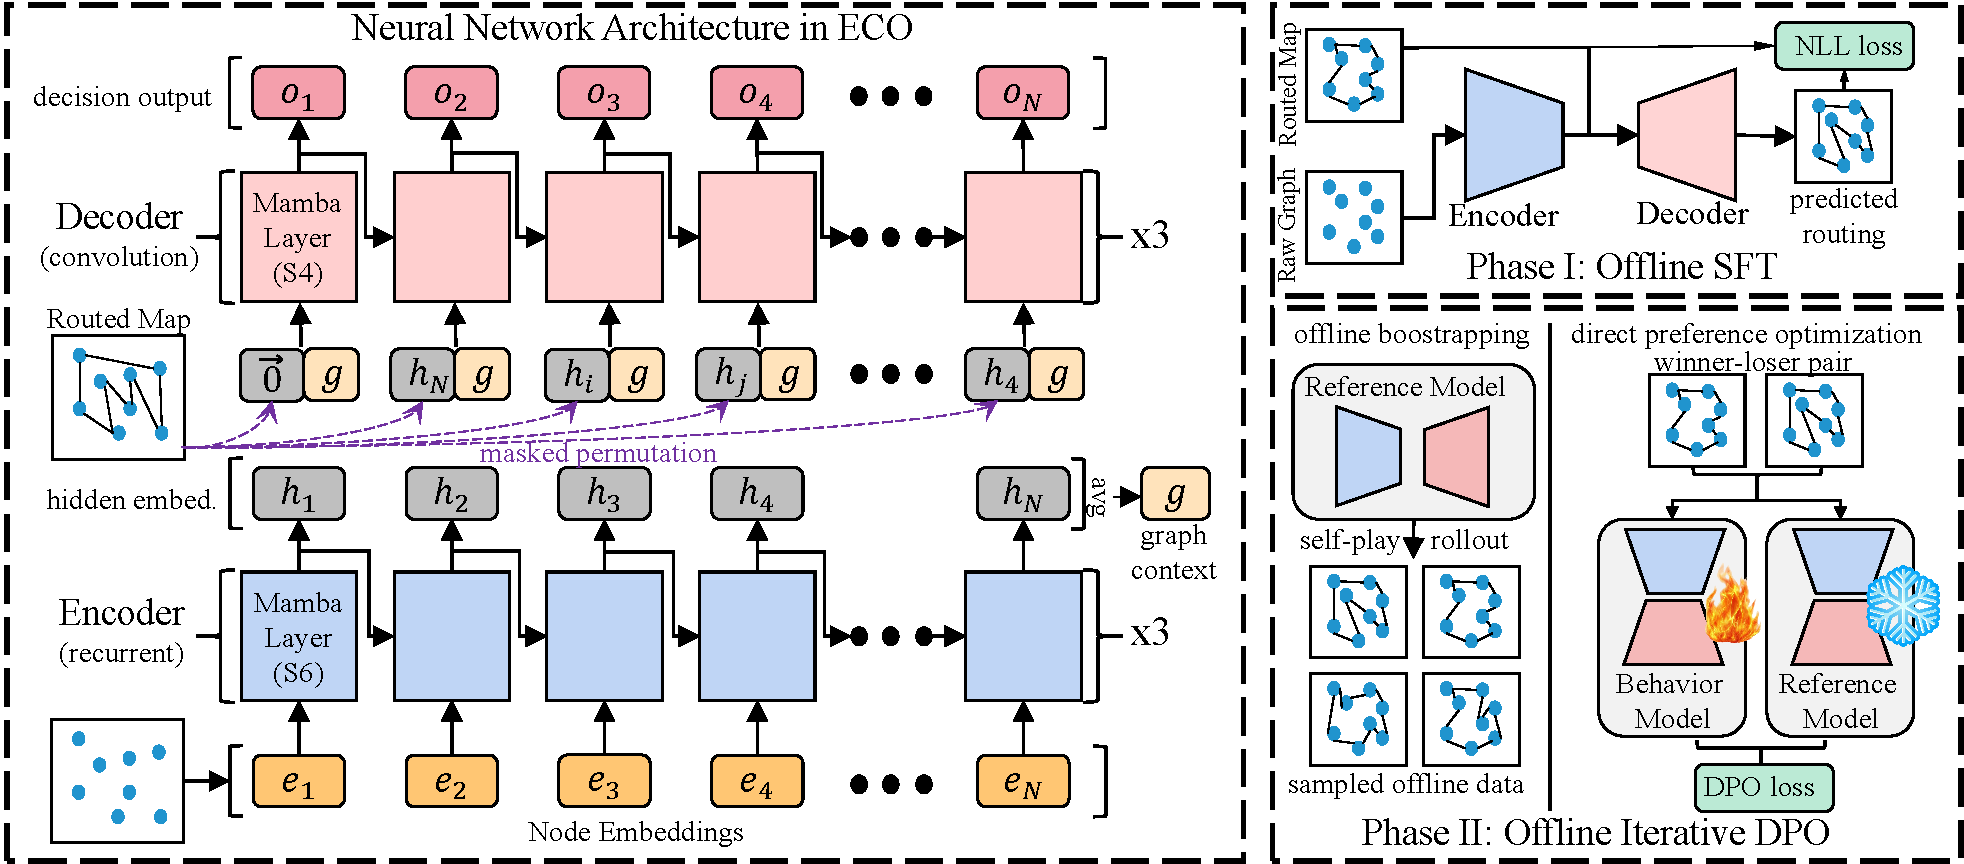
\includegraphics[width=0.98\linewidth]{figure/eco_method_fig.pdf}

\caption{The core designs and workflow of our ECO. \textbf{Left}: The Mamba-based Encoder-Decoder architecture proposed to facilitate offline NCO training. \textbf{Right}: The two-phase offline learning with a SFT warm-up as quick knowledge adaption and an iterative preference learning to further enhance performance.}
\label{fig:method}
\vspace{-15pt}
\end{figure*}
\vspace{-5pt}
\subsection{Preference Learning}

% Policy gradient-based reinforcement learning, such as REINFORCE and PPO, currently dominates the NCO training paradigm. However, these methods are often sensitive to baseline design and suffer from low sample efficiency in later training stages. In parallel, within the field of Large Language Model (LLM) alignment, Rafailov et al. introduced DPO \cite{10}. DPO demonstrates that policies can be optimized to match human preferences via a simple classification loss, effectively bypassing complex reward modeling and the instability inherent in online PPO. Subsequent works like ReST \cite{11} and Self-Rewarding LM \cite{12} further validate the potential of iterative optimization using self-generated samples of varying quality. This concept aligns perfectly with the intrinsic nature of NCO, where solutions of differing quality (specifically, "preferred" versus "rejected" trajectories) are readily obtainable for a given instance. This paper explores the integration of DPO into NCO training for the first time, aiming to replace traditional scalar rewards with contrastive learning signals to achieve more robust policy optimization.

Classic reinforcement learning~(RL), either value-based methods~\cite{DQN} or policy-gradient methods~\cite{REINFORCE,A2C,PPO}, relies on well-defined, hand-crafted reward functions to ensure training effectiveness. Recently, a general consensus has emerged that such rewarding schemes often lead to \emph{reward hacking}~\cite{reward-hacking}, optimizing the designer's proxy metrics rather than the actual human intent. To address this, Ouyang et al. proposed reinforcement learning from human feedback~(RLHF)~\cite{9}, where a reward model is explicitly trained from pairwise human feedback comparisons and subsequently optimized using policy-gradient methods.

Following RLHF, DPO~\cite{10} introduced critical technical modifications to streamline this bi-stage workflow. Specifically, DPO demonstrates that the constrained policy optimization problem can be solved analytically, allowing policies to be optimized to match preferences via a simple classification loss. This effectively bypasses the complexity of explicit reward modeling and the instability inherent in online PPO. Building on this, subsequent works like ReST~\cite{11} and Self-Rewarding LM~\cite{12} further validated the potential of iterative optimization using self-generated samples of varying quality. Consequently, two promising directions are currently being widely explored in the community: bootstrapping strategies~\cite{11,12} for data efficiency and learning objective reformulation~\cite{KTO,ORPO} for robustness.

Leveraging this paradigm, we adopt DPO as the base learner for our framework. While the application of DPO to NCO has been explored in concurrent works~\cite{dpo-nco-1,dpo-nco-2,dpo-nco-3}, our work advances this direction by addressing the unique data challenges in combinatorial optimization. We introduce: 1) a two-phase training protocol that incorporates a high-quality supervised warm-up to stabilize the DPO routine, and 2) a heuristic-guided bootstrapping strategy to relieve the burden of offline data generation, the details of which are elaborated in Sec.~\ref{sec:3.3}.



\vspace{-10pt}
\section{Method}
\vspace{-5pt}
The core idea of our ECO is illustrated in Figure~\ref{fig:method}. In ECO, we have established a well-defined offline learning paradigm to leverage high-quality offline trajectory data for efficient NCO training. on the top of such offline paradigm, we have introduced a mixed Mamba-architecture which synergizes both long-sequence modeling and efficient inference. We further design an effective two-phase training workflow to assure robust convergence under the offline setting. In the subsequent sections, we provide detailed elaboration on every aspects of ECO in a step-by-step way.

% designed a scalable and generic framework designed for sequence modeling in NCO's setting. We first provide a unified problem formulation for routing-style CO tasks. We then detail our linear-complexity architecture based on SSM and conclude with our novel training paradigm: Iterative Preference Optimization with Local Search Distillation.
\vspace{-5pt}
\subsection{Problem Formulation}
We consider a general class of combinatorial optimization problems that can be formulated as finding an optimal permutation or sequence of nodes on a graph. Let $G = (V, E)$ be a graph where $V = \{v_1, \dots, v_N\}$ represents a set of $N$ nodes (e.g., cities in TSP, customers in CVRP) characterized by feature vectors $X = \{x_1, \dots, x_N\}$ (e.g., coordinates, demands). The goal is to generate a sequence $\pi = (\pi_1, \dots, \pi_T)$ of indices from $\{1, \dots, N\}$ that satisfies specific feasibility constraints $\Omega$ (e.g., visiting every node exactly once, capacity limits) while minimizing a cost objective $\mathcal{C}(\pi | G)$. The problem is formally defined as:

\begin{equation}
   \pi^* = \arg\min_{\pi \in \Omega} \mathcal{C}(\pi | G).
\end{equation}
We model this as a probabilistic sequence generation task using a parameterized policy $p_\theta(\pi | X)$. By decomposing the joint probability via the chain rule, the probability of a solution $\pi$ is:
\begin{equation}
    p_\theta(\pi | X) = \prod_{t=1}^T p_\theta(\pi_t | \pi_{<t}, X),
\end{equation}
where $\pi_{<t}$ denotes the partial solution constructed up to step $t-1$. Our objective is to optimize parameters $\theta$ such that the expected cost $\mathbb{E}_{\pi \sim p_\theta}[\mathcal{C}(\pi|X)]$ is minimized.
\vspace{-5pt}
\subsection{Offline Training Paradigm}\label{sec:3.3}

Traditional  RL methods for CO, such as REINFORCE with a greedy rollout baseline, often suffer from high variance and training instability. Inspired by recent advances in LLM alignment, we propose a robust two-phase training strategy: a warm-up phase using supervised learning and a continuous policy improvement phase using iterative DPO~\cite{10}.

\subsubsection{Phase I: Supervised Fine-Tuning (SFT)}

This phase provides the policy model with a basic understanding of TSP constraints and local optimality, we perform behavior cloning on high-quality solutions.

\textbf{Data Generation:} We generate a dataset $\mathcal{D}_{\text{SFT}}$ using the LKH-3 solver (or nearest neighbor heuristics for rapid initialization).

\textbf{Objective:} We minimize the Negative Log-Likelihood (NLL) of the expert trajectories $\pi^*$:
\vspace{-10pt}
\begin{equation}
    \mathcal{J}_{\text{SFT}}(\theta) = - \mathbb{E}_{(X, \pi^*) \sim \mathcal{D}_{\text{SFT}}} \left[ \sum_{t=1}^N \log p_\theta(\pi_t^* | \pi_{<t}^*, X) \right]
\end{equation}
\vspace{-10pt}
\subsubsection{Phase II: Iterative Direct Preference Optimization (DPO)}

The core of our training is the Iterative DPO algorithm. Unlike PPO, DPO optimizes the policy directly from preference data without training a separate value function (Critic), significantly reducing memory overhead and training complexity.

\textbf{Preference Pair Construction:} In each iteration $k$, we generate a dataset of preference pairs. For a given instance $X$, we sample $K$ solutions $\{y_1, \dots, y_K\}$ using the current policy $\pi_{\theta}$. To construct a pair $(y_w, y_l)$:
\textbf{Winner ($y_w$):} The trajectory with the shorter tour length. \textbf{Loser ($y_l$):} The trajectory with the longer tour length.

\textbf{DPO Objective:} We optimize the policy $\pi_\theta$ to maximize the margin between the likelihood of the winner and the loser, constrained by a reference model $\pi_{\text{ref}}$ (the policy from the previous iteration). The loss function is:
\vspace{-5pt}
\begin{equation}
\begin{split}
\mathcal{L}_{\text{DPO}}(\theta; \pi_{\text{ref}}) = 
- \mathbb{E}_{(X, y_w, y_l)} \bigg[ 
& \log \sigma \bigg( \beta \log \frac{\pi_\theta(y_w|X)}{\pi_{\text{ref}}(y_w|X)} \\
& - \beta \log \frac{\pi_\theta(y_l|X)}{\pi_{\text{ref}}(y_l|X)} \bigg) \bigg]
\end{split}
\end{equation}

where $\sigma$ is the sigmoid function and $\beta$ is a temperature parameter controlling the deviation from the reference model.

\textbf{Iterative Refinement:} Instead of a static reference model, we update $\pi_{\text{ref}} \leftarrow \pi_{\theta}$ every $T$ steps. This iterative approach allows the model to progressively "climb" the quality landscape, generating increasingly better reference distributions for subsequent self-improvement cycles.

\subsubsection{Enhancing Preference Contrast via Local Search}

In the standard DPO framework, preference pairs are constructed solely from model-sampled trajectories. As training progresses, the policy tends to generate solutions with similar quality, resulting in narrow reward margins ($|L(y_w) - L(y_l)| \to 0$). This leads to vanishing gradients and hinders the model's ability to distinguish subtle structural improvements.

To address this, we introduce an LS-Augmented Preference Construction mechanism. This strategy integrates a lightweight local search operator $\mathcal{T}_{\text{LS}}$ (e.g., 2-opt or 3-opt) into the data generation process to amplify the quality contrast and distill local optimization capabilities into the neural policy.

Mechanism:
For a subset of instances in each iteration, given a model-generated solution $y_{\text{raw}} \sim \pi_\theta(\cdot|X)$, we apply the local search operator to obtain an improved version: $y_{\text{refined}} = \mathcal{T}_{\text{LS}}(y_{\text{raw}})$. We then construct the preference pair $(y_w, y_l)$ strictly as:
\vspace{-5pt}
\begin{equation}
    y_w = y_{\text{refined}}, \quad y_l = y_{\text{raw}}
\end{equation}
\vspace{-5pt}
Crucially, since $\mathcal{T}_{\text{LS}}$ guarantees $L(y_{\text{refined}}) \le L(y_{\text{raw}})$, this construction provides a strictly cleaner and stronger supervision signal.



\textbf{Margin Amplification:} By manually widening the performance gap between the winner and the loser, we increase the magnitude of the implicit reward difference $\hat{r}_\theta(y_w) - \hat{r}_\theta(y_l)$. This results in sharper gradients, accelerating convergence in plateau regions.

\textbf{Operator Distillation:} This process effectively treats the DPO objective as a distillation loss. By consistently preferring the LS-refined solution over the raw output, the model implicitly learns the underlying geometric manipulations (e.g., untangling crossing edges) performed by the 2-opt/3-opt operator, effectively "internalizing" the local search into the Mamba encoder-decoder weights without requiring explicit execution during inference.


\subsection{Mixed Mamba-based Architecture}
Transformer-based NCO models (e.g., AM~\cite{3} and POMO~\cite{4}), if without further software or hardware-level optimization~(e.g., KV cache~\cite{kv-cache}, flash-attention~\cite{flashattention}), fall short in addressing large scale~(long-sequence) CO problems. To address this, we propose a tailored neural network architecture~(as shown in Figure~\ref{fig:method}), including 1) a recurrent mode Mamba-based encoder to enable economical memory utilization and long-sequence correlation extraction. By using such as mixed Mamba-based architecture, we maximize both the long-sequence modeling ability in encoder and parallel rollout/inference throughput in decoder. We detail this architecture as belows, with its computation steps and complexity analysis.

\subsubsection{Recurrent Mamba Encoder}

The encoder transforms the raw coordinate sequence into rich contextual node embeddings. Unlike the standard Transformer encoder which computes an $N \times N$ attention map, our encoder utilizes stacked Mamba layers\footnote{https://github.com/state-spaces/mamba}.

\textbf{Input Projection:} The coordinates $x_i$ are projected into a $D$-dimensional latent space via a linear transformation: 
\begin{equation}
    e_i = W_{\text{in}} x_i + b_{\text{in}}.
\end{equation}
\textbf{Mamba Layers:} We use Mamba layers with S6 setting~(see the end of Sec.~\ref{sec:2.2}). This input-dependent setting helps the encoder to extract spatial dependence across a long sequence of nodes in a large scale CO problems. We denote the $L=3$ layers' parameters as $M_{enc}^{(1)}$, $M_{enc}^{(2)}$ and $M_{enc}^{(3)}$. Then following the per-layer computation in Eq.~\ref{eq:s4}, we recurrently compute hidden embeddings of all nodes:
\begin{equation}
    H = M_{enc}^{(3)} \circ M_{enc}^{(2)} \circ M_{enc}^{(1)}(E),
\end{equation}
where $E$ is all node embeddings $e_i$ and $H:\{h_i\}_{i=1}^{N}$ are the obtained hidden embeddings for all nodes in the CO problems. We additionally compute a global graph embedding $g = mean(H)$ as a context information used for the decoding phase. Since we adopt Mamba with S6 setting, the recurrent mode is used, which leverages the parallel scan algorithm to reduce the recurrent complexity.

% The input sequence $H^{(0)}$ is passed through $L$ layers of Mamba blocks. Each block employs a Selective State Space Model. For a sequence input $x(t)$, the continuous SSM is defined as:
% \begin{equation}
%     h'(t) = \mathbf{A}h(t) + \mathbf{B}x(t), \quad y(t) = \mathbf{C}h(t)
% \end{equation}
% The Mamba block discretizes this process using the Zero-Order Hold (ZOH) method, allowing the model to be computed efficiently via parallel scans. By stacking these blocks, the encoder captures long-range dependencies between cities without the heavy memory footprint of self-attention.

% \textbf{Output:} The final node embeddings $H^{(L)} = \{h_1, \dots, h_N\}$ encapsulate both local geometric features and global graph topology.


\subsubsection{Convolutional Mamba Decoder}
\textbf{Input Preparation.} Since ECO operates in an offline setting, the decoder is always paired with offline data, which is a routed map as shown in Figure~\ref{fig:method}. Given the hidden embeddings $H:\{h_i\}_{i=1}^{N}$, We first use the routed map as permutation mask to re-order the embeddings in $H$ as the visiting order in the routed map, and obtain the permuted embeddings $H^\prime:\{h^\prime_i\}_{i=1}^{N}$. Then, the input prepared as:
\begin{equation}
    h^\prime_i = h^\prime_i + g, \quad i=1,...,N,
\end{equation}
where $g$ is the global context we obtained from the encoder. In this way, we inject an explicit problem-specific context into the decoding phase, to help inform the decoder problem-specific features.

\textbf{Decoding.} We use Mamba layers with S4 setting~(see Sec.~\ref{sec:2.2} and Eq.~\ref{eq:s4-kernal}) to facilitate parallel decoding, hence maximizing the decoding efficiency. We denote the $L=3$ layers' parameters as $M_{dec}^{(1)}$, $M_{dec}^{(2)}$ and $M_{dec}^{(3)}$ and obtain decision output $O:\{o_i\}_{i=1}^{N}$ by:
\begin{equation}
    O = M_{dec}^{(3)} \circ M_{dec}^{(2)} \circ M_{dec}^{(1)}(H^\prime).
\end{equation}
The logits in $O$ are masked to prevent revisiting cities and normalized via Softmax to produce the selection probability $p(\pi_t | \pi_{<t}, X)$.

% We depart from the standard attention-based decoder by introducing a recurrence-based SSM decoder. This design maintains the efficiency of the encoder and eliminates the $O(N)$ complexity per decoding step associated with Cross-Attention.

% \textbf{State Maintenance:} The decoder maintains a hidden state $s_t$ updated via the SSM recurrent rule. At time step $t$, given the embedding of the previously selected node $h_{\pi_{t-1}}$, the state is updated as:

% \begin{equation}
%     s_t = \text{SSM}_{\text{step}}(s_{t-1}, h_{\pi_{t-1}})
% \end{equation}

% \textbf{Bilinear Scoring Mechanism:} To decide the next city $\pi_t$, we compute a compatibility score (logit) between the current decoder state $s_t$ and all unvisited city embeddings $h_j$:
% \begin{equation}
%     u_{j,t} = (W_q s_t)^T W_k h_j, \quad \forall j \in \{1, \dots, N\} \setminus \pi_{<t}
% \end{equation}

% \textbf{Probabilistic Output:} The logits are masked to prevent revisiting cities and normalized via Softmax to produce the selection probability $p(\pi_t | \pi_{<t}, X)$.

\subsubsection{Algorithm Complexity}
Based on the unified encoder-decoder pipeline, we briefly compare the algorithm complexity of the classic Transformer NCO architecture and our proposed Mixed Mamba-based architecture. For the Transformer, the memory complexity in the encoder is quadratic $O(N^2)$ (due to the self-attention matrix) , and the computational complexity in the decoder is generally quadratic $O(N^2)$ (scaling linearly per step due to cross-attention). In contrast, for Mamba, the memory complexity in the encoder is linear $O(N)$ (enabled by parallel scan), and the computational complexity in the decoder is linear $O(N)$ (due to the fixed-size recurrent state update). This offers a significant advantage for scalable NCO deployment. Our experimental results (Sec.~\ref{sec:4.2.2}) validate this analysis.



\section{Experiment}




\begin{table*}[t]
\centering
\caption{
\textbf{Performance comparison on TSP and CVRP instances of varying sizes.} 
We report the average objective value (Obj.), the average optimality gap (Gap) relative to the ground truth, and the total inference time (Time).
\textbf{Concorde}, \textbf{LKH-3} and \textbf{HGS} are used as the ground truth solvers for TSP and CVRP, respectively (indicated by 0.00\% Gap). 
For learning-based methods, the best results are highlighted in \textbf{bold}, and the second-best results are \underline{underlined}.
}
\label{tab:main_results}
\resizebox{\textwidth}{!}{% 如果表格过宽，自动缩放以适应页面
\begin{tabular}{l|ccc|ccc|ccc|ccc}

\toprule
\multicolumn{1}{c|}{\multirow{2}{*}{Method}} & \multicolumn{3}{c|}{\cellcolor{tspgreen}TSP200} & \multicolumn{3}{c|}{\cellcolor{tspgreen}TSP500} & \multicolumn{3}{c|}{\cellcolor{tspgreen}TSP1000} & \multicolumn{3}{c}{\cellcolor{tspgreen}TSP5000} \\
 & \cellcolor{tspgreen}Obj.$\downarrow$ & \cellcolor{tspgreen}Gap$\downarrow$ & \cellcolor{tspgreen}Time$\downarrow$ & \cellcolor{tspgreen}Obj.$\downarrow$ & \cellcolor{tspgreen}Gap$\downarrow$ & \cellcolor{tspgreen}Time$\downarrow$ & \cellcolor{tspgreen}Obj.$\downarrow$ & \cellcolor{tspgreen}Gap$\downarrow$ & \cellcolor{tspgreen}Time$\downarrow$ & \cellcolor{tspgreen}Obj.$\downarrow$ & \cellcolor{tspgreen}Gap$\downarrow$ & \cellcolor{tspgreen}Time$\downarrow$ \\ \midrule
Concorde & 10.72 & 0.00\% & 3.0m & 16.55 & 0.00\% & 37.6m & 23.12 & 0.00\% & 7.9h & 50.96 & 0.00\% & 18.4h \\
LKH-3 & 10.72 & 0.00\% & 0.8m & 16.55 & 0.00\% & 1.5m & 23.12 & 0.00\% & 24m & 50.96 & 0.00\% & 9.6h \\ \midrule
AM & 11.03 & 2.89\% & 0.3m & 21.24 & 28.34\% & 1.4m & 35.18 & 52.16\% & 2.2m & 96.37 & 89.11\% & 5.7m \\
POMO & 10.97 & 2.33\% & 0.2m & 20.85 & 25.98\% & 1.0m & 32.94 & 42.47\% & 1.6m & 87.79 & 72.27\% & 4.8m \\
CNF & 10.80 & 0.74\% & 1.5m & 17.29 & 4.47\% & 3.3m & 25.19 & 8.95\% & 7.7m & 56.53 & 10.93\% & 11.1m \\
GFlowNet-HBG & \underline{10.78} & 0.56\% & 0.1m & \underline{17.05} & 3.02\% & 0.5m & \underline{24.42} & 5.62\% & 1.3m & \underline{54.67} & 7.28\% & 3.7m \\
ECO & 10.96 & 2.23\% & 0.1m & 17.73 & 7.12\% & 0.4m & 25.33 & 9.55\% & 0.9m & 57.02 & 11.89\% & 2.5m \\
\textbf{ECO(Local search)} & \textbf{10.76} & \textbf{0.37\%} & \textbf{0.1m} & \textbf{16.98} & \textbf{2.59\%} & \textbf{0.4m} & \textbf{24.24} & \textbf{4.84\%} & \textbf{0.9m} & \textbf{53.76} & \textbf{5.49\%} & \textbf{2.5m} \\ \midrule
 & \multicolumn{3}{c|}{\cellcolor{cvrpblue}CVRP100} & \multicolumn{3}{c|}{\cellcolor{cvrpblue}CVRP200} & \multicolumn{3}{c|}{\cellcolor{cvrpblue}CVRP500} & \multicolumn{3}{c}{\cellcolor{cvrpblue}CVRP1000} \\
 & \cellcolor{cvrpblue}Obj.$\downarrow$ & \cellcolor{cvrpblue}Gap$\downarrow$ & \cellcolor{cvrpblue}Time$\downarrow$ & \cellcolor{cvrpblue}Obj.$\downarrow$ & \cellcolor{cvrpblue}Gap$\downarrow$ & \cellcolor{cvrpblue}Time$\downarrow$ & \cellcolor{cvrpblue}Obj.$\downarrow$ & \cellcolor{cvrpblue}Gap$\downarrow$ & \cellcolor{cvrpblue}Time$\downarrow$ & \cellcolor{cvrpblue}Obj.$\downarrow$ & \cellcolor{cvrpblue}Gap$\downarrow$ & \cellcolor{cvrpblue}Time$\downarrow$ \\ \midrule
HGS & 15.56 & 0.00\% & 0.4m & 19.63 & 0.00\% & 1.0m & 37.15 & 0.00\% & 6.1m & 63.26 & 0.00\% & 13.7m \\ \midrule
AM & 16.73 & 7.51\% & 0.2m & 21.33 & 8.64\% & 0.8m & 47.36 & 27.39\% & 2.0m & 104.40 & 65.03\% & 3.9m \\
POMO & 16.15 & 3.79\% & 0.2m & 20.47 & 4.26\% & 0.6m & 46.13 & 24.17\% & 1.4m & 100.19 & 58.37\% & 2.1m \\
CNF & 15.85 & 1.86\% & 0.3m & 20.08 & 2.31\% & 1.8m & 38.51 & 3.64\% & 4.3m & 66.94 & 5.82\% & 8.7m \\
GFlowNet-HBG & \underline{15.70} & 0.91\% & 0.1m & \underline{20.01} & 1.96\% & 0.2m & \underline{38.19} & 2.81\% & 0.7m & \underline{65.09} & 2.89\% & 1.7m \\
ECO & 15.87 & 1.99\% & 0.1m & 20.13 & 2.57\% & 0.2m & 38.61 & 3.94\% & 0.6m & 67.11 & 6.08\% & 1.2m \\
\textbf{ECO(Local search)} & \textbf{15.69} & \textbf{0.86\%} & \textbf{0.1m} & \textbf{20.33} & \textbf{1.77\%} & \textbf{0.2m} & \textbf{38.21} & \textbf{2.85\%} & \textbf{0.6m} & \textbf{65.08} & \textbf{2.87\%} & \textbf{1.8m} \\ \bottomrule
\end{tabular}%
}
\end{table*}




\subsection{Experimental Setup}


\textbf{Problem Instances:} Following standard generation protocols \cite{3}, we synthesized datasets for both TSP and CVRP. To evaluate scalability, we tested problem sizes of $N \in \{200, 500, 1000, 5000\}$. All reported results represent the average performance computed over 1,000 independent test instances.


\textbf{Model Configuration:} The model embedding dimension is set to 128. Both the Mamba-based encoder and decoder consist of 3 layers. For the DPO training stability, we set the KL penalty coefficient $\beta$ to 0.3 and the sampling size $K$ to 32. The reference model is updated every 10 iterations. We utilize the Adam optimizer with a learning rate of $5 \times 10^{-4}$ and L2 regularization.

\textbf{Training Protocol:} Our training pipeline proceeds in two stages. The first stage is a warm-up phase (Supervised Fine-Tuning), where the model is trained for 10 epochs on 100,000 instances labeled by the LKH solver to acquire foundational heuristic knowledge. The second stage implements DPO training using offline data generation. Here, we enhance the learning signal by integrating a local search operator, with a mixing ratio $\alpha = 0.3$ for the optimized data. All experiments were conducted on a single NVIDIA A800 GPU (80GB).



\textbf{Baselines:} To rigorously validate our approach, we benchmark against two categories of methods: (1) Traditional solvers, including LKH \cite{lkh}, HGS \cite{HGS} and Concorde \cite{concorde2006} ; and (2) Representative and state-of-the-art NCO methods, specifically AM \cite{3},POMO \cite{4},CNF \cite{CNF}, and GFlowNet (HBG) \cite{GFlowNet}.
\vspace{-5pt}
\subsection{Experimental Analysis}
\vspace{-5pt}
To systematically address the core objectives of this study, we structure our experimental analysis around the following three Research Questions (RQs):

RQ1 (Scalability and Quality): Can ECO maintain solution quality comparable to mainstream Transformer-based NCO methods on large-scale instances while significantly reducing inference latency?

RQ2 (Efficiency Mechanism): Does the proposed Mamba architecture empirically demonstrate linear GPU memory scaling and superior throughput advantages over Attention mechanisms in long-sequence tasks?

RQ3 (Component Effectiveness): What are the individual contributions of the offline DPO paradigm, the warm-up strategy, and heuristic bootstrapping to the final model performance?

\subsubsection{Main Results Analysis (Responds to RQ1)}
\begin{figure*}[!ht]  % 核心修改：[!ht]替代[H]
\centering
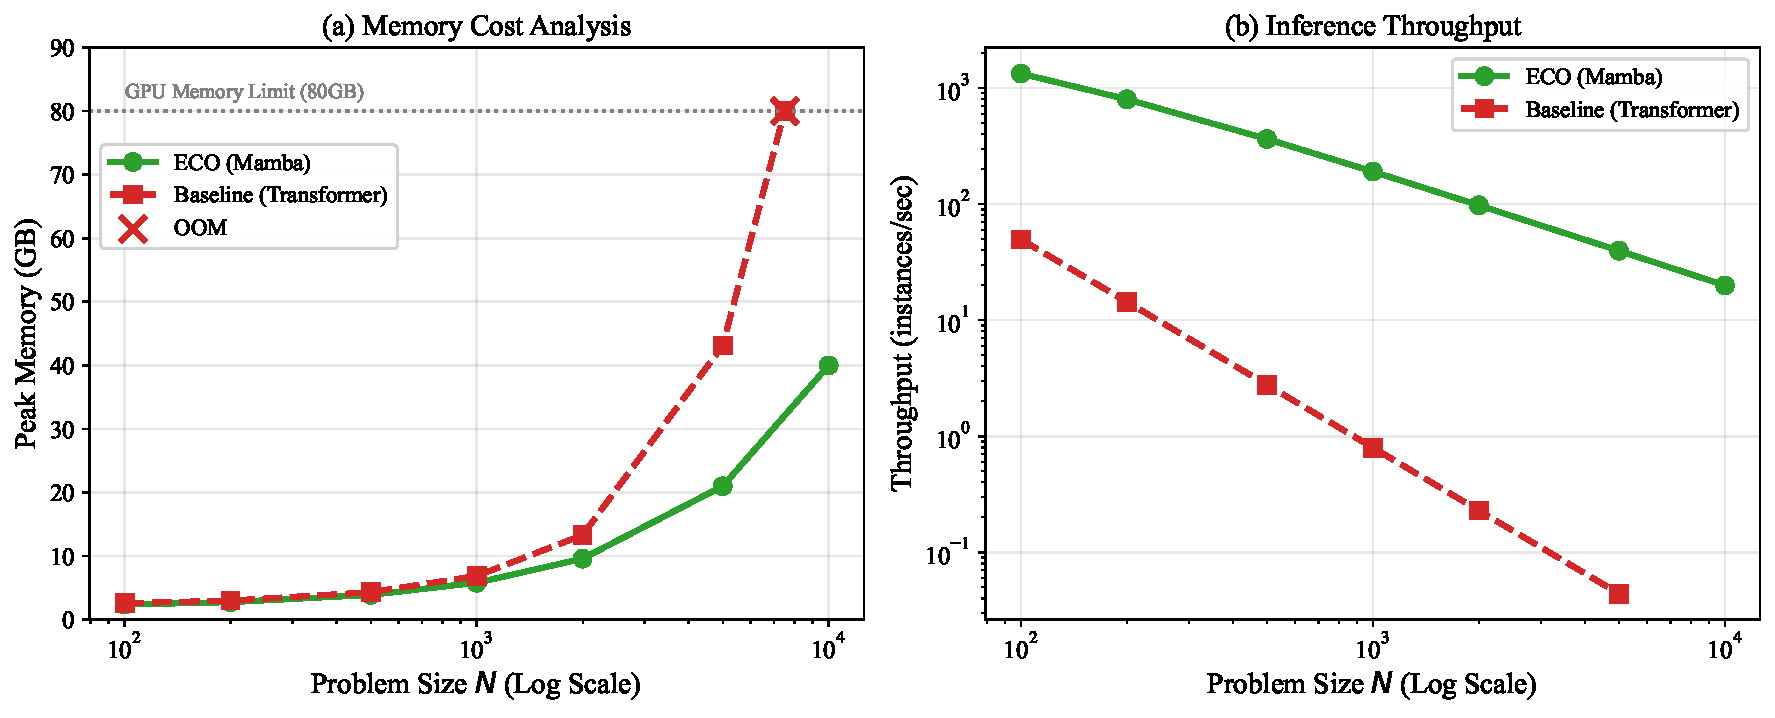
\includegraphics[width=\linewidth]{figure/efficiency_analysis_strict.pdf}
\vspace{-0.3cm} 

\caption{
\textbf{Scalability and Efficiency Analysis on NVIDIA A800 GPU (80GB RAM).} 
We perform a stress test comparing the resource consumption of ECO (Mamba-based) against the Transformer baseline across problem sizes $N$ ranging from 100 to 10,000 (log scale).
\textbf{(a) Peak Memory Usage:} The baseline exhibits characteristic quadratic growth ($O(N^2)$) due to the self-attention mechanism, triggering an Out-Of-Memory (OOM) error at $N=10,000$. In contrast, ECO maintains a near-linear memory profile ($O(N)$) owing to Mamba's fixed-size recurrent state, enabling scalable inference well within hardware limits.
\textbf{(b) Inference Throughput:} ECO demonstrates orders-of-magnitude higher throughput (note the log scale on the y-axis) compared to the baseline. The performance gap widens significantly as $N$ increases, validating the computational efficiency advantage of our proposed SSM architecture for large-scale NCO tasks.
}
\label{fig:efficiency}
\vspace{-0.4cm}
\end{figure*}
Table \ref{tab:main_results} presents the comparative performance on TSP and CVRP instances ranging from $N=200$ to $N=5000$. Our analysis yields two primary conclusions regarding the scalability and learning efficacy of ECO:

\textbf{Robust Performance on Large-Scale Instances:} The most critical validation of our approach is observed on the massive-scale instances (TSP5000/CVRP1000). As shown in Table 1, traditional Transformer-based baselines (AM, POMO) suffer from significant performance degradation as the problem size increases, with optimality gaps deteriorating to $89.11\%$ and $72.27\%$ on TSP5000. This collapse is largely attributed to the difficulty of training attention mechanisms to capture global dependencies on such large graphs. In contrast, ECO maintains consistent high performance, achieving a competitive gap of $11.89\%$ on TSP5000. This result confirms that our Mamba-based architecture, combined with the proposed training paradigm, successfully scales to manage the complexity of thousands of nodes, overcoming the scalability bottlenecks inherent in previous NCO solvers.

\textbf{Internalizing Local Search Capabilities via DPO:} A key driver of ECO's superior performance is the integration of Local Search (LS) into the DPO training phase. Rather than serving merely as a post-hoc repair operator, the LS-augmented data generation provides high-quality "winner" trajectories ($y_w$) for the preference pairs. By optimizing the policy to distinguish between the raw model output and the LS-refined solution, ECO effectively distills the geometric optimization logic of 2-opt/3-opt operators directly into the neural network weights. This "internalization" process sharpens the learning signal, enabling the model to generate structurally superior solutions autonomously. When a lightweight LS is optionally applied during inference (ECO(Local Search)), the performance is further refined, bridging the gap to the specialized LKH-3 solver ($5.49\%$ gap on TSP5000) while retaining a substantial speed advantage.

\textbf{Inference Latency and Practicality:} ECO demonstrates a decisive advantage in computational efficiency. On TSP5000, ECO completes inference in just 2.5 minutes, representing a speedup of orders of magnitude compared to constructive heuristics and iterative baselines. This establishes ECO as a highly practical solver for time-sensitive, large-scale industrial routing scenarios where traditional solvers typically require hours of computation.
\vspace{-5pt}
\subsubsection{Efficiency and Throughput Analysis (Responds to RQ2)}
\label{sec:4.2.2}
\vspace{-5pt}
% 无需额外改其他代码，仅修改定位参数


To rigorously isolate the efficiency gains attributed to the proposed SSM architecture, we conducted a controlled stress test. We implemented a Control Variate Baseline by replacing the Mamba backbone within the ECO framework with a standard Transformer architecture (mimicking the Attention Model), while keeping all other data processing and inference pipelines identical.

\textbf{GPU Memory Scaling Analysis:} We monitored the peak GPU memory consumption across problem sizes $N \in \{100, \dots, 10000\}$. To accurately capture the architectural growth rate ($O(N)$ vs. $O(N^2)$), we standardized the inference batch size to 8 for all measurements.

\textbf{Results:} As illustrated in Figure \ref{fig:efficiency} (Left), the Transformer baseline exhibits a quadratic memory explosion, triggering an Out-Of-Memory (OOM) error on the A800 (80GB) GPU at approximately $N=7000$. Conversely, ECO maintains a strictly linear memory growth profile. Even at $N=10,000$, the memory footprint remains well within hardware limits (approx. 40GB). This confirms that the fixed-size recurrent state of the Mamba encoder-decoder effectively resolves the memory bottleneck preventing Transformer-based models from scaling.

\textbf{Limit-State Throughput Testing:} To evaluate the maximum processing capacity suitable for industrial deployment, we adopted a Maximal Utilization Protocol for throughput testing. Instead of a fixed batch size, we dynamically maximized the inference batch size for each model and problem size until the GPU memory limit was reached.

\textbf{Results:} Figure \ref{fig:efficiency} (Right) reports the throughput (instances/second) on a logarithmic scale. While the Transformer's throughput plummets for large $N$ due to the necessity of reducing batch sizes to accommodate the massive attention matrices, ECO sustains high throughput levels. Specifically, at $N=5000$, ECO achieves a throughput orders of magnitude higher than the baseline. This performance gap highlights that the linear memory complexity of ECO not only saves VRAM but also unlocks the ability to process significantly larger batches in parallel, maximizing GPU utilization.

\subsection{Ablation Study (Responds to RQ3)}
\begin{table}[t]
    \caption{Ablation study on TSP1000. We report the average Optimality Gap (Gap) relative to the ground truth and the Total Training Time. ``--'' indicates that the model failed to converge or exhibited instability. The best results are highlighted in \textbf{bold}.}
    \vspace{-5pt}
    \label{tab:ablation}
    \begin{center}
    \begin{small}
    \begin{sc}
    % 使用 resizebox 确保表格宽度严格适配单栏宽度 (0.48\textwidth 或 \columnwidth)
    \resizebox{\columnwidth}{!}{
        \begin{tabular}{llcc}
            \toprule
            Variant & Components & Gap (\%) $\downarrow$ & Time $\downarrow$ \\
            \midrule
            \textbf{ECO (Full)}    & SFT + DPO + LS   & \textbf{4.84} & \textbf{10.2h} \\
            w/o LS Boot.  & SFT + DPO        & 9.55          & 9.5h \\
            w/o SFT       & DPO + LS         & $>20.0$       & -- \\
            Online PPO    & Online RL        & 4.88          & 34.5h \\
            \bottomrule
        \end{tabular}
    }    
    \end{sc}
    \end{small}
    \end{center}
    \vspace{-25pt}
\end{table}
To verify the contribution of the Offline DPO paradigm, Local Search (LS) Bootstrapping, and supervised warm-up (SFT), we conducted an ablation study on TSP1000. Table \ref{tab:ablation} summarizes the results across four variants.



% 确保在导言区引入了这些宏包
% \usepackage{booktabs}
% \usepackage{graphicx}



\textbf{The Necessity of Heuristic Bootstrapping (Signal Quality):} A critical hypothesis of our work is that standard self-play suffers from "reward sparsity" in late training stages, where the model struggles to generate solutions significantly better than its current policy. As shown in Table 2, removing the LS augmentation (w/o LS Bootstrapping) leads to a distinct performance drop, with the optimality gap increasing from $4.84\%$ to $9.55\%$. Without the injection of high-quality solutions via local search, the preference margins $L(y_l) - L(y_w)$ become vanishingly small. In the DPO loss landscape, this results in weak gradients, causing the model to stagnate in local optima. The LS operator effectively acts as a "guidance compass," providing a strictly superior $y_w$ that forces the policy to learn the geometric transformations required to escape these local optima.

\textbf{Offline DPO vs. Online PPO (Paradigm Efficiency):} We challenge the dominance of Online RL in NCO by comparing ECO against a standard Online PPO baseline utilizing the same Mamba architecture. While PPO can eventually converge, it requires significantly more wall-clock time ($T_{PPO} \approx 3 \times T_{ECO}$) to reach comparable performance. Furthermore, ECO (Full) achieves a better final convergence gap. This validates the efficiency of the Offline paradigm. Online RL is bottlenecked by the interaction loop—generating fresh samples on-policy for every update step—which severely limits GPU utilization. In contrast, ECO's offline data generation (coupled with parallelized Mamba inference) maximizes computational throughput. Moreover, DPO's direct optimization of the policy distribution avoids the instability associated with training a separate Value Network (Critic) in PPO.

\textbf{The Role of Warm-up (The "Cold Start" Problem):} The w/o SFT variant fails to yield meaningful results, exhibiting an optimality gap of $>20\%$ and unstable training curves. This confirms that DPO is highly sensitive to the quality of the reference model $\pi_{ref}$. If initialized randomly, both the reference policy and the current policy generate effectively random tours. Consequently, the preference pairs $(y_w, y_l)$ contain no structural logic (i.e., $y_w$ is better than $y_l$ by pure chance, not by merit), leading to noisy gradients that derail the optimization. The SFT phase is therefore indispensable, providing the "topological common sense" required to bootstrap the preference learning process.


\section{Conclusion}

In this paper, we introduced ECO, a scalable NCO framework that fundamentally rethinks the efficiency bottlenecks of current neural solvers. By synergizing a linear-complexity Mamba architecture with an offline self-play paradigm, ECO effectively breaks the quadratic memory barrier and low-throughput constraints of Transformer-based online methods. Extensive experiments on TSP and CVRP confirm that ECO delivers competitive solution quality at a fraction of the computational cost, enabling practical inference on instances with thousands of nodes. Our findings suggest that shifting towards hardware-aware architectures and stable offline alignment strategies is a promising path for the next generation of large-scale combinatorial optimization.











\section*{Impact Statement}

This paper presents work whose goal is to advance the field of Machine
Learning. There are many potential societal consequences of our work, none
which we feel must be specifically highlighted here.
\bibliography{ref}
\bibliographystyle{icml2026}

%%%%%%%%%%%%%%%%%%%%%%%%%%%%%%%%%%%%%%%%%%%%%%%%%%%%%%%%%%%%%%%%%%%%%%%%%%%%%%%
%%%%%%%%%%%%%%%%%%%%%%%%%%%%%%%%%%%%%%%%%%%%%%%%%%%%%%%%%%%%%%%%%%%%%%%%%%%%%%%
% APPENDIX
%%%%%%%%%%%%%%%%%%%%%%%%%%%%%%%%%%%%%%%%%%%%%%%%%%%%%%%%%%%%%%%%%%%%%%%%%%%%%%%
%%%%%%%%%%%%%%%%%%%%%%%%%%%%%%%%%%%%%%%%%%%%%%%%%%%%%%%%%%%%%%%%%%%%%%%%%%%%%%%
\newpage
\appendix
\onecolumn
\section{ Theoretical Analysis of Iterative DPO for Combinatorial Optimization}
In this appendix, we provide a theoretical derivation of the Direct Preference Optimization (DPO) objective specifically within the context of Combinatorial Optimization (CO). We further analyze the gradient dynamics to explain why the iterative update of the reference model promotes convergence towards optimal solutions.

\subsection{Derivation of the DPO Objective for TSP}
The Traveling Salesperson Problem (TSP) can be formulated as a Reinforcement Learning problem where the objective is to maximize the expected reward (minimize tour length) subject to a KL-divergence constraint. This constraint ensures the policy does not deviate excessively from a reference policy $\pi_{\text{ref}}$, stabilizing the training.

\textbf{The RL Objective:} Let $R(\pi, X) = -L(\pi, X)$ be the reward function (negative tour length). The objective is to find the optimal policy $\pi^*$ maximizing:
\begin{equation}
    \max_{\pi} \mathbb{E}_{X \sim \mathcal{D}, \pi \sim \pi(\cdot|X)} \left[ R(\pi, X) \right] - \beta \mathbb{D}_{KL}(\pi(\cdot|X) || \pi_{\text{ref}}(\cdot|X)),
\end{equation}
where $\beta$ is the regularization coefficient.
%%%%%%%%%%%%%%%%%%%%%%%%%%%%%%%%%%%%%%%%%%%%%%%%%%%%%%%%%%%%%%%%%%%%%%%%%%%%%%%
%%%%%%%%%%%%%%%%%%%%%%%%%%%%%%%%%%%%%%%%%%%%%%%%%%%%%%%%%%%%%%%%%%%%%%%%%%%%%%%
The Closed-Form Solution: As shown in previous works, the optimal solution to this constrained maximization problem takes the form of a Gibbs distribution:

\begin{equation}
    \pi^*(y|X) = \frac{1}{Z(X)} \pi_{\text{ref}}(y|X) \exp\left( \frac{R(y, X)}{\beta} \right),
\end{equation}
where $Z(X) = \sum_{y'} \pi_{\text{ref}}(y'|X) \exp(R(y', X)/\beta)$ is the partition function.

\textbf{Eliminating the Partition Function:} By rearranging the equation above, we can express the reward function $R$ in terms of the optimal policy, the reference policy, and the partition function:

\begin{equation}
    R(y, X) = \beta \log \frac{\pi^*(y|X)}{\pi_{\text{ref}}(y|X)} + \beta \log Z(X).
\end{equation}
This mapping is crucial because $Z(X)$ depends only on the instance $X$, not on the specific path $y$.

\textbf{Modeling Preferences via Bradley-Terry:} In our framework, we do not train an explicit Reward Model. Instead, we use paired data $(y_w, y_l)$ where $L(y_w) < L(y_l)$, implying $y_w \succ y_l$. Assuming the preference distribution follows the Bradley-Terry model:

\begin{equation}
    p(y_w \succ y_l | X) = \sigma(R(y_w, X) - R(y_l, X)).
\end{equation}

Substituting the expression for $R(y, X)$ derived above, the partition function terms $\beta \log Z(X)$ cancel out:

\begin{equation}
    R(y_w, X) - R(y_l, X) = \beta \log \frac{\pi^*(y_w|X)}{\pi_{\text{ref}}(y_w|X)} - \beta \log \frac{\pi^*(y_l|X)}{\pi_{\text{ref}}(y_l|X)}.
\end{equation}

Optimizing the negative log-likelihood of this probability yields the DPO loss $\mathcal{L}_{\text{DPO}}$ used in our method.

\subsection{Gradient Analysis and Optimization Dynamics}
To understand why DPO is effective for TSP, we analyze the gradient of the loss function with respect to the network parameters $\theta$. The gradient is given by:

\begin{equation}
    \nabla_\theta \mathcal{L}_{\text{DPO}} = - \beta \mathbb{E}_{(X, y_w, y_l)} \left[ \underbrace{\sigma(\hat{r}_\theta(y_l) - \hat{r}_\theta(y_w))}_{\text{Error Term}} \left( \underbrace{\nabla_\theta \log \pi_\theta(y_w|X)}_{\text{Reinforce Winner}} - \underbrace{\nabla_\theta \log \pi_\theta(y_l|X)}_{\text{Suppress Loser}} \right) \right],
\end{equation}
where $\hat{r}_\theta(y) = \beta \log \frac{\pi_\theta(y|X)}{\pi_{\text{ref}}(y|X)}$ is the implicit reward.

\textbf{Intuition for CO:}

\textbf{Implicit Reward Shaping:} The term $\hat{r}_\theta(y_w) - \hat{r}_\theta(y_l)$ acts as a dynamic margin. The model updates its weights to increase the likelihood of the shorter path $y_w$ relative to the reference model, while decreasing the likelihood of $y_l$.

\textbf{Automatic Curriculum via the Error Term:} The scaling factor $\sigma(\hat{r}_\theta(y_l) - \hat{r}_\theta(y_w))$ essentially represents the "probability of making a mistake" (classifying the longer path as better).

If the model is confident and correct ($y_w$ is much more likely than $y_l$), this term approaches 0, and the gradient vanishes (preventing overfitting).

If the model is incorrect ($y_l$ is more likely), the term approaches 1, applying a strong gradient to correct the behavior.

This provides a natural, sample-efficient curriculum that focuses learning on "hard" comparisons, which is critical for fine-grained optimization in TSP.


\subsubsection{Convergence of Iterative DPO (Iterative Reference Updates)}

Standard DPO relies on a static $\pi_{\text{ref}}$. However, in Combinatorial Optimization, the static reference limits the exploration capability, as the KL constraint prevents the policy from drifting too far from an initially sub-optimal heuristic.



Our Iterative DPO strategy updates $\pi_{\text{ref}}^{(t+1)} \leftarrow \pi_{\theta}^{(t)}$ periodically. This can be viewed as a Generalized Expectation-Maximization (GEM) process:

\textbf{E-Step (Sampling):} By updating $\pi_{\text{ref}}$, we effectively reset the "search radius" of the KL constraint. The new reference distribution $\pi_{\text{ref}}^{(t+1)}$ is concentrated on better solutions found in iteration $t$.

\textbf{M-Step (Optimization):} We optimize $\pi_\theta$ to find solutions better than the new reference.

Since $L(y_w) < L(y_l)$ is grounded in the absolute metric of Euclidean distance (unlike subjective human preferences), the preference signal is noise-free.
Let $\mathcal{S}_t$ be the set of high-probability paths under $\pi^{(t)}$. The iterative update ensures that $\mathbb{E}_{y \sim \pi^{(t+1)}}[L(y)] \leq \mathbb{E}_{y \sim \pi^{(t)}}[L(y)]$ as long as the optimizer can find a $y_w$ in the local neighborhood of $\pi^{(t)}$ such that $L(y_w) < L(y_l)$. This mimics a population-based evolutionary strategy where the population (distribution) progressively shifts towards the global optimum.

\section{Detailed Implementation Settings}

To ensure the reproducibility of our results, we provide the detailed hyperparameter settings for both the neural architecture and the training phases.


\subsection{Network Architecture}
Our Mamba-based Encoder-Decoder follows the official implementation configurations of Mamba~\cite{mamba}. The specific architectural hyperparameters are detailed in Table \ref{tab:arch_params}.
% 正文区单栏表格代码

\begin{table}[h]
\caption{Hyperparameters of the Mixed Mamba Architecture.}
\label{tab:arch_params}
\centering  % 单栏轻量居中，适配table环境
\begin{sc}
\begin{tabular}{p{8cm}c}  % 单栏核心：第一列固定6cm宽度，第二列居中
\toprule
Parameter & Value \\
\midrule
Embedding Dimension ($D$) & 128 \\
Number of Layers ($L$) & 3 \\
Mamba State Dimension ($d_{state}$) & 16 \\
Mamba Conv Kernel Size ($d_{conv}$) & 4 \\
Mamba Expansion Factor ($E$) & 2 \\
Feed-Forward Network (FFN) Ratio & 4 \\
Normalization & RMSNorm \\
\bottomrule
\end{tabular}
\end{sc}
\end{table}

\subsection{Baseline Configurations and Reproducibility}

To ensure a fair comparison, all baselines were evaluated on the same hardware environment (Single NVIDIA A800 GPU). We utilized the official open-source implementations for the learning-based methods: 

\begin{itemize}
    \item \textbf{Attention Model (AM)} and \textbf{POMO}: We used the implementation from the widely adopted \texttt{RL4CO} library\footnote{\url{https://github.com/ai4co/rl4co}}, maintaining their default hyperparameters.
    \item \textbf{GFlowNet-HBG}: We utilized the official code provided by \cite{GFlowNet}, training the model with their recommended settings for 24 hours.
    \item \textbf{CNF}: We reproduced the results using the official code from \cite{CNF}, ensuring the flow-matching steps were consistent with their paper.
\end{itemize}

For traditional solvers: 
\begin{itemize}
    \item \textbf{Concorde}: We used the PyConcorde wrapper.
    \item \textbf{LKH-3}: We used the official binary with standard parameters (runs=1, max-trials=10000).
\end{itemize}

\subsection{Data Generation and Local Search Details}
Following standard NCO protocols \cite{3}, problem instances for both TSP and CVRP are generated by sampling $N$ node coordinates uniformly from the unit square $[0, 1]^2$. For CVRP, demands are sampled uniformly from discrete values $\{1, \dots, 9\}$, and capacities are set to $20$, $30$, $40$, and $50$ for $N=20, 50, 100, 200$ respectively. For larger scales ($N \ge 500$), capacities are scaled linearly.


In the Bootstrapping DPO phase, we employ  2-opt/3-opt local search operator to refine the raw model outputs. To balance efficiency and solution quality during data generation:
\begin{itemize}
\item We implement a First Improvement strategy rather than Best Improvement to reduce computational overhead.
\item The maximum number of 2-opt iterations is capped at $N$ (linear to problem size) to prevent excessive runtime during the offline data generation process.
\item This operator is implemented using Numba JIT compilation to ensure it does not become a bottleneck in the training pipeline.
\item During DPO training, we incorporate preference pairs enhanced by local search to strengthen the learning signal. Specifically, these augmented pairs constitute 20\% of the total training data.
\end{itemize}

\subsection{Algorithm Pseudocode}
We provide the detailed training procedure of ECO in Algorithm \ref{alg:eco_training}. The framework consists of two phases: Supervised Fine-Tuning (SFT) warm-up and Iterative Direct Preference Optimization (DPO) with Heuristic Bootstrapping.

\begin{algorithm}[h]
   \caption{ECO: Efficient Combinatorial Optimization Training Framework}
   \label{alg:eco_training}
\begin{algorithmic}[1]
   \STATE {\bfseries Input:} Training instances $\mathcal{X}$, Expert Solver (LKH/Heuristic) $\mathcal{H}$, Local Search Operator $\mathcal{T}_{LS}$
   \STATE {\bfseries Hyperparameters:} Learning rates $\eta_{SFT}, \eta_{DPO}$, Sampling size $K$, Mixing ratio $\alpha$, Reference update freq $M$, KL coefficient $\beta$
   \STATE {\bfseries Initialize:} Policy parameters $\theta$, Reference model $\theta_{ref} \leftarrow \theta$
   
   \STATE \COMMENT{\textcolor{blue}{\textbf{Phase I: Supervised Warm-up (SFT)}}}
   \STATE Generate expert demonstrations $\mathcal{D}_{SFT} = \{(x, \pi^*) \mid x \in \mathcal{X}, \pi^* = \mathcal{H}(x)\}$
   \FOR{epoch $= 1$ {\bfseries to} $E_{SFT}$}
       \FOR{batch $B \subset \mathcal{D}_{SFT}$}
           \STATE Compute Loss $\mathcal{L}_{SFT}(\theta) = - \frac{1}{|B|} \sum_{(x, \pi^*) \in B} \log p_\theta(\pi^* | x)$
           \STATE Update $\theta \leftarrow \theta - \eta_{SFT} \nabla_\theta \mathcal{L}_{SFT}$
       \ENDFOR
   \ENDFOR

   \STATE \COMMENT{\textcolor{blue}{\textbf{Phase II: Iterative DPO with LS Bootstrapping}}}
   \STATE Initialize $\theta_{ref} \leftarrow \theta$
   \FOR{iteration $t = 1$ {\bfseries to} $T_{DPO}$}
       \STATE Sample batch of instances $X_{batch} \subset \mathcal{X}$
       \STATE Initialize preference buffer $\mathcal{D}_{pref} \leftarrow \emptyset$
       
       \FOR{instance $x \in X_{batch}$}
           \STATE Sample $K$ solutions $Y = \{y_1, \dots, y_K\}$ using current policy $\pi_\theta(\cdot|x)$
           
           \STATE \COMMENT{\textit{Heuristic Bootstrapping Strategy}}
           \IF{random() $< \alpha$}
               \STATE Select a candidate $y_{raw} \in Y$
               \STATE Apply Local Search: $y_{refined} \leftarrow \mathcal{T}_{LS}(y_{raw})$
               \STATE Set pair: $y_w \leftarrow y_{refined}, \quad y_l \leftarrow y_{raw}$ \quad \COMMENT{Strictly better signal}
           \ELSE
               \STATE Evaluate costs $\{L(y) \mid y \in Y\}$
               \STATE Set pair: $y_w \leftarrow \arg\min_{y \in Y} L(y), \quad y_l \leftarrow \arg\max_{y \in Y} L(y)$
           \ENDIF
           
           \STATE Add $(x, y_w, y_l)$ to $\mathcal{D}_{pref}$
       \ENDFOR
       
       \STATE \COMMENT{\textit{DPO Update}}
       \STATE Compute Implicit Rewards: $\hat{r}_\theta(y) = \beta \log \frac{\pi_\theta(y|x)}{\pi_{ref}(y|x)}$
       \STATE Compute Loss $\mathcal{L}_{DPO}(\theta) = - \mathbb{E}_{(x,y_w,y_l) \sim \mathcal{D}_{pref}} \left[ \log \sigma \left( \hat{r}_\theta(y_w) - \hat{r}_\theta(y_l) \right) \right]$
       \STATE Update $\theta \leftarrow \theta - \eta_{DPO} \nabla_\theta \mathcal{L}_{DPO}$
       
       \STATE \COMMENT{\textit{Iterative Reference Update}}
       \IF{$t \mod M == 0$}
           \STATE Update Reference Model: $\theta_{ref} \leftarrow \theta$
       \ENDIF
   \ENDFOR
   
   \STATE {\bfseries Output:} Optimized parameters $\theta$
\end{algorithmic}
\end{algorithm}

\end{document}

% This document was modified from the file originally made available by
% Pat Langley and Andrea Danyluk for ICML-2K. This version was created
% by Iain Murray in 2018, and modified by Alexandre Bouchard in
% 2019 and 2021 and by Csaba Szepesvari, Gang Niu and Sivan Sabato in 2022.
% Modified again in 2023 and 2024 by Sivan Sabato and Jonathan Scarlett.
% Previous contributors include Dan Roy, Lise Getoor and Tobias
% Scheffer, which was slightly modified from the 2010 version by
% Thorsten Joachims & Johannes Fuernkranz, slightly modified from the
% 2009 version by Kiri Wagstaff and Sam Roweis's 2008 version, which is
% slightly modified from Prasad Tadepalli's 2007 version which is a
% lightly changed version of the previous year's version by Andrew
% Moore, which was in turn edited from those of Kristian Kersting and
% Codrina Lauth. Alex Smola contributed to the algorithmic style files.
